\documentclass[10pt]{beamer}
%%
\usepackage{pgfpages}
\usepackage{graphicx}
\usepackage{ulem}
\usepackage{color}
\usepackage{fancyvrb}
\usepackage{listings}
\usepackage{hyperref}
\hypersetup{colorlinks=true}

\lstset{
  language=R,
  % basicstyle=\scriptsize\ttfamily,
  basicstyle=\scriptsize\ttfamily,
  % commentstyle=\ttfamily\color{gray},
  % numbers=none,
%  backgroundcolor=\color{white},
  showspaces=false,
  showstringspaces=false,
%  showtabs=false,
%  frame=single,
  % tabsize=2,
  % captionpos=b,
  breaklines=true
  % breakatwhitespace=false,
%  title=\lstname,
  % escapeinside={},
  % keywordstyle={},
  % morekeywords={}
}

% get rid of junk
\usetheme{default}
\beamertemplatenavigationsymbolsempty
\hypersetup{pdfpagemode=UseNone} % don't show bookmarks on initial view
% font
\usefonttheme{professionalfonts}
\usefonttheme{serif}
% page number
\setbeamertemplate{footline}{%
  \raisebox{5pt}{\makebox[\paperwidth]{\hfill\makebox[20pt]{\color{gray}
        \scriptsize\insertframenumber}}}\hspace*{5pt}}
% add a bit of space at the top of the notes page
\addtobeamertemplate{note page}{\setlength{\parskip}{12pt}}

\setbeamertemplate{blocks}[rounded][shadow=true]

\AtBeginSection{
  \begin{frame}
    \begin{center}
      {\Large \insertsection}
    \end{center}
  \end{frame}
}

\newcommand{\df}{{\it data.frame} }
\newcommand{\gr}{{\it GRanges} }
\newcommand{\dfs}{{\it data.frames} }
\newcommand{\mat}{{\it matrix} }

\title{HGSS R Workshop : Tidyverse and Bioconductor}
\author{Jean Monlong}
\institute{Human Genetics department}
\date{March 26, 2018}

\begin{document}


\begin{frame}[fragile]{Before we begin}
  \begin{block}{}
    \begin{enumerate}
    \item Open R/Rstudio or whatever you use.
    \item Prepare a folder for the workshop and set it as working directory.
    \item Install packages and download the data.
    \end{enumerate}
  \end{block}
  \bigskip
  
  Instructions and slides available at \url{https://github.com/jmonlong/HGSS_Rworkshops/} (in the {\sf Advanced-Tidyverse-Bioconductor-2018} folder}).

\end{frame}

%%%%%%%%%%%%%%%%%%%%
%% Title Slide
\begin{frame}
  \centering
  \titlepage
  \begin{minipage}{.4\textwidth}
    \includegraphics[width=.8\linewidth]{../imgs/hgssLogo-black.png}
  \end{minipage}
  \hspace{.1\textwidth}
  \begin{minipage}{.4\textwidth}
    \includegraphics[width=\linewidth]{../imgs/McGill-Logo1.png}
  \end{minipage}
  \bigskip
  
  {\scriptsize Sponsored by the McGill Initiative in Computational Medicine (MiCM)}
\end{frame}

\begin{frame}{Today's topic}
  \begin{block}{}
    \begin{itemize}
    \item Manipulating, analyzing and visualizing large \df in the \href{https://www.tidyverse.org/}{Tidyverse}.
    \item Tricks: cleaner and faster code.
      \medskip
      
    \item Access and manipulate genomics ranges.
    \item Tricks: Gene enrichment analysis, heatmaps.
    \end{itemize}
  \end{block}

  \begin{alertblock}{Disclaimer}
    \begin{itemize}
    \item Some things might be too technical. Follow what you can.
    \item Feel free to interrupt or suggest other ways.
    \end{itemize}
  \end{alertblock}

\begin{block}{}
    \begin{itemize}
    \item Lunch break: 12:15pm - 1:15pm
    \end{itemize}
  \end{block}
  
  
\end{frame}

%%%%%%%%%%%%%%%%%%
%%%%%%%%%%%%%%%%%%
%%%%%%%%%%%%%%%%%%
%%\section{Manipulating, analyzing and visualizing large \df in the Tidyverse}

\begin{frame}[fragile]{{\it data.table} package and {\sf fread}}
  \begin{block}{{\sf fread} function}
    \begin{description}
    \item[+] Very fast.
    \item[+] Usually no need for additional parameters.
    \item[-] Has its specific format ({\it data.table})...
    \item[+] ... which can be converted into \df.
    \item[+] Very fast.
    \end{description}
  \end{block}
  \begin{exampleblock}{Example}
    \begin{lstlisting}
library(data.table)
myDT = fread("myFile.tsv")
myDF = as.data.frame(myDT)

myDT = fread("gunzip -c myFile.tsv.gz")
\end{lstlisting}
  \end{exampleblock}
\end{frame}

\begin{frame}[fragile]{Exercise}
  \begin{enumerate}
  \item Read the Gencode file (\verb!gencodeForWorkshop.tsv.gz!) with \verb!read.table!.
  \item Same with \verb!fread!.
  \item Have a look at the data.
  \item For each gene type, compute
    \begin{itemize}
    \item the number of genes
    \item the average gene size
    \item the proportion of genes larger than 1 Kbp
    \end{itemize}
    {\it Hint: one \df with the results.}
  \item 4. again but for chr Y only.
  \end{enumerate}
\end{frame}

\begin{frame}[fragile]{Avoid loops, use {\sf sapply/lapply}}
  \begin{block}{}
    \begin{description}
    \item[+] Avoid manual init/update of objects.
    \item[+] No temporary object polluting the environment.
    \item[+] More optimized.
    \item[+] Easy to parallelize.
    \item[-] More painful to debug.
    \item[-] An error and everything must be computed again.
    \end{description}
  \end{block}
  \begin{block}{}
  \begin{lstlisting}
perm.l = lapply(1:1000, function(ii){
  data.frame(perm=ii, est=..SOMETHING..)
})

perm.df = do.call(rbind, perm.l)
## or
perm.df = as.data.frame(rbindlist(perm.l))
  \end{lstlisting}
  \end{block}
\end{frame}

\begin{frame}[fragile]{Minimize copy-pasting, use {\sf functions}}
  \begin{block}{}
    \begin{description}
    \item[+] Easier to propagate changes.
    \item[+] Easier to reuse in another analysis.
    \item[+] Cleaner/smaller code.
    \end{description}
  \end{block}
  \begin{block}{}
  \begin{lstlisting}
superFun <- function(df, arg1, opt2=0){
  ## Something with df, arg1 and opt2
  return(XXX)
}
  \end{lstlisting}
  \end{block}
  \begin{alertblock}{Exercise}
    Improve the previous exercise with {\sf functions}.
  \end{alertblock}
\end{frame}

\begin{frame}[fragile]{Parallel processing}
  \begin{block}{Easiest solution with {\it parallel} package}
    \begin{itemize}
    \item Using \verb!mclapply! instead of \verb!lapply!.
    \item \verb!mc.cores=! the number of processors to use.
    \end{itemize}
  \end{block}
  \begin{exampleblock}{Example}
\begin{lstlisting}
perm.l = mclapply(1:1000, function(ii){
  data.frame(perm=ii, est=..SOMETHING..)
}, mc.cores=4)
\end{lstlisting}
  \end{exampleblock}
  \begin{alertblock}{Exercise}
    Parallelize the previous exercise.
  \end{alertblock}
\end{frame}

\begin{frame}{The Tidyverse}
  \centering
  \url{https://www.tidyverse.org/}
  \bigskip
  
  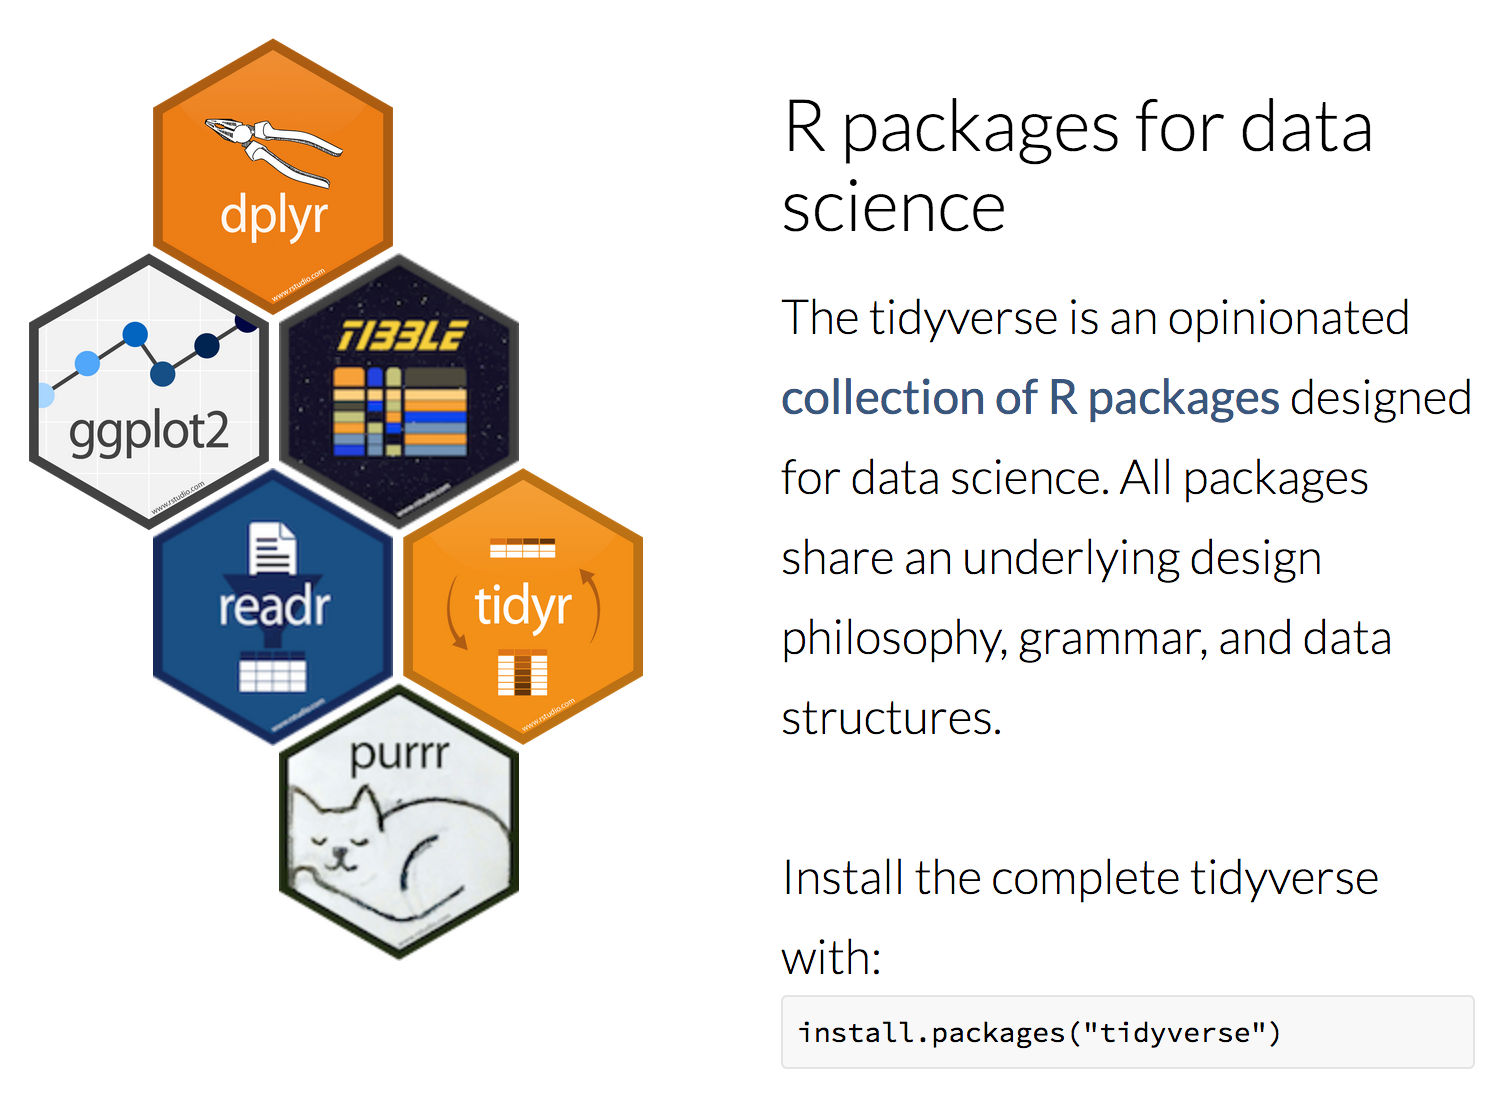
\includegraphics[height=.8\textheight]{../imgs/tidyverse.png}
  
\end{frame}

\begin{frame}[fragile, shrink=19]{\dfs}
  \begin{block}{}
    \begin{itemize}
    \item Mix between \mat and {\it list}
    \item Array form.
    \item Columns can have different data types.
    \end{itemize}
  \end{block}
  \begin{columns}
    \begin{column}{.5\textwidth}
      \begin{block}{\mat}
\begin{Verbatim}[commandchars=\\\{\}]
      samp1 samp2 samp3
gene1  \color{blue}-1.3  -1.8  -4.1\color{black}
gene2  \color{blue}-1.5  -1.2   4.9\color{black}
\end{Verbatim}
      \end{block}
    \end{column}
    \begin{column}{.5\textwidth}
      \begin{block}{\df}
\begin{Verbatim}[commandchars=\\\{\}]
 gene sample expression
\color{red}gene1  samp1       \color{blue}-1.3\color{black}
\color{red}gene2  samp1       \color{blue}-1.5\color{black}
\color{red}gene1  samp2       \color{blue}-1.8\color{black}
\color{red}gene2  samp2       \color{blue}-1.2\color{black}
\color{red}gene1  samp3       \color{blue}-4.1\color{black}
\color{red}gene2  samp3       \color{blue} 4.9\color{black}
\end{Verbatim}
      \end{block}
    \end{column}
  \end{columns}
  \begin{block}{Pros/Cons}
    \begin{columns}
      \begin{column}{.5\textwidth}
        \begin{description}
        \item[+] Dense representation of large data.
        \item[-] Accepts only one data type.
        \item[-] \underline{manual} combination with other information often required.
        \end{description}
      \end{column}
      \begin{column}{.5\textwidth}
        \begin{description}
        \item[+] Flexible.
        \item[+] Accepts several data types.
        \item[+] Can represent all the data needed for an analysis.
        \item[-] Takes more space/memory due to repetitions.
        \end{description}
      \end{column}
    \end{columns}
  \end{block}
\end{frame}

\begin{frame}[fragile]{{\it dplyr} package}
  \begin{block}{``A Grammar of Data Manipulation''}
    {\it dplyr} provides functions which can be combined for data manipulation.
    \begin{description}
    \item[mutate] add a new column using others.
    \item[filter] filter rows (similar as \verb!subset! function).
    \item[select] select specific columns only.
    \item[arrange] order rows using specific columns.
    \item[group\_by] groups rows according to specific columns.
    \item[summarize] summarizes each group of rows.
    \item[do] applies a function to a group of rows.
    \end{description}
  \end{block}
  \begin{block}{}
    \begin{description}
      \item[+] Works with pipes.
      \item[+] Fast.
      \item[-] Has its own format {\it tbl\_df}...
      \item[+] ... which is almost the same as \df.
    \end{description}
  \end{block}
\end{frame}

\begin{frame}[fragile]{Pipes are cool !}
  \begin{block}{}
    \begin{itemize}
    \item Pipe functions instead of embedding them.
    \item More readable.
    \item Easier to combine several functions.
    \item Avoid temporary objects.
    \item Pipe argument \verb!%>%!.
    \end{itemize}
  \end{block}
  \begin{exampleblock}{Example}
\begin{Verbatim}[commandchars=\\\{\}]
head(sort(round(sqrt(myVec))))
myVec \color{blue}%>%\color{black} sqrt \color{blue}%>%\color{black} round \color{blue}%>%\color{black} sort \color{blue}%>%\color{black} head

head(\color{blue}sort(\color{red}round(\color{black}sqrt(myVec)\color{red},digits=3)\color{blue},decreasing=TRUE)\color{black},10)
myVec \color{blue}%>%\color{black} sqrt \color{blue}%>%\color{black} round(digits=3) \color{blue}%>%\color{black}
                        sort(decreasing=TRUE) \color{blue}%>%\color{black} head(10)
\end{Verbatim}
  \end{exampleblock}
\end{frame}

\begin{frame}[fragile]{Grouping rows}
  \begin{block}{Operation by block}
    \begin{itemize}
    \item Using \verb!group_by()! function.
    \item Further operations are applied separately per group of rows.
    \end{itemize}
  \end{block}
  \begin{exampleblock}{Example}
\begin{lstlisting}
myDF %>% group_by(colA) %>% summarize(colB.mean=mean(colB))

myDF %>% group_by(colA, colB) %>% summarize(nbAB=n())

myDF %>% group_by(colAB) %>% summarize(nbAB=n()) %>%
                 ungroup %>% arrange(desc(nbAB)) %>% head
\end{lstlisting}
  \end{exampleblock}
  \begin{block}{Tips}
    \begin{itemize}
    \item \verb!n()! gives the number of rows in the group.
    \item \verb!ungroup! removes groups.
    \item \verb!desc()! means descending order (in \verb!arrange()!).
    \end{itemize}
  \end{block}
\end{frame}

\begin{frame}[fragile]{Exercise}
  \begin{enumerate}
  \item Print the top 10 genes with the most exons.
    \bigskip
  \item Same exercise as before with \verb!group_by! instead of \verb!lapply!.
    \begin{itemize}
    \item For each gene type, compute
      \begin{itemize}
      \item the number of genes
      \item the average gene size
      \item the proportion of genes larger than 1 Kbp
      \end{itemize}
    \item Idem for chr Y only.
    \end{itemize}
    \bigskip
  \item Idem with \verb!summarize! (i.e. no functions).
  \end{enumerate}
\end{frame}

\begin{frame}{{\sf ggplot2} package}
  \begin{block}{Introduction}
    A package to construct pretty and/or complex graphs. Many aspects of the graph are arranged automatically but everything can be customized. Easy layers addition.
  \end{block}

  \includegraphics[height=.6\textheight]{../imgs/example-ggplot2.pdf}
  \includegraphics[height=.6\textheight,page=2]{../imgs/example-ggplot2.pdf}

\end{frame}

\begin{frame}[fragile, shrink=10]{{\sf ggplot2}}
  \begin{block}{Input : \df}
    \begin{itemize}
    \item Each row represents one {\it "observation"}.
    \item Columns represent the different information about the {\it "observations"}.
    \end{itemize}
  \end{block}

  \begin{block}{Concept}
    \begin{itemize}
    \item Start with a \verb!ggplot(...)! and the input \df.
    \item \verb!aes(...)! defines how to use the input's columns.
    \item Add layers : \verb!geom_*(...)!, \verb!scale_*(...)!, ...
    \end{itemize}
  \end{block}

  \begin{exampleblock}{Example}
\begin{Verbatim}[commandchars=\\\{\}]
library(ggplot2)
\color{blue}ggplot(\color{red}myDf\color{black}\color{blue}, aes(\color{black}x=\color{red}colA\color{black}, y=\color{red}colB\color{black}, colour=\color{red}colC\color{black}, linetype=\color{red}colD\color{black}\color{blue}))
   + geom_point() + geom_line() + scale_y_log10()
\end{Verbatim}
  \end{exampleblock}

  \begin{block}{Useful online resources}
    \begin{itemize}
    \item \url{http://docs.ggplot2.org/current/}
    \item \url{http://www.cookbook-r.com/Graphs/}
    \end{itemize}
  \end{block}

\end{frame}

\begin{frame}{Exercise}
  \begin{enumerate}
  \item Show the distribution of the gene size (histogram), colored by gene type.
  \item Show for each chromosome the number of genes, colored by gene type.
    \bigskip
    
  \item[$\divideontimes$] Plot the proportion of gene types in each chromosome.

    \centering
    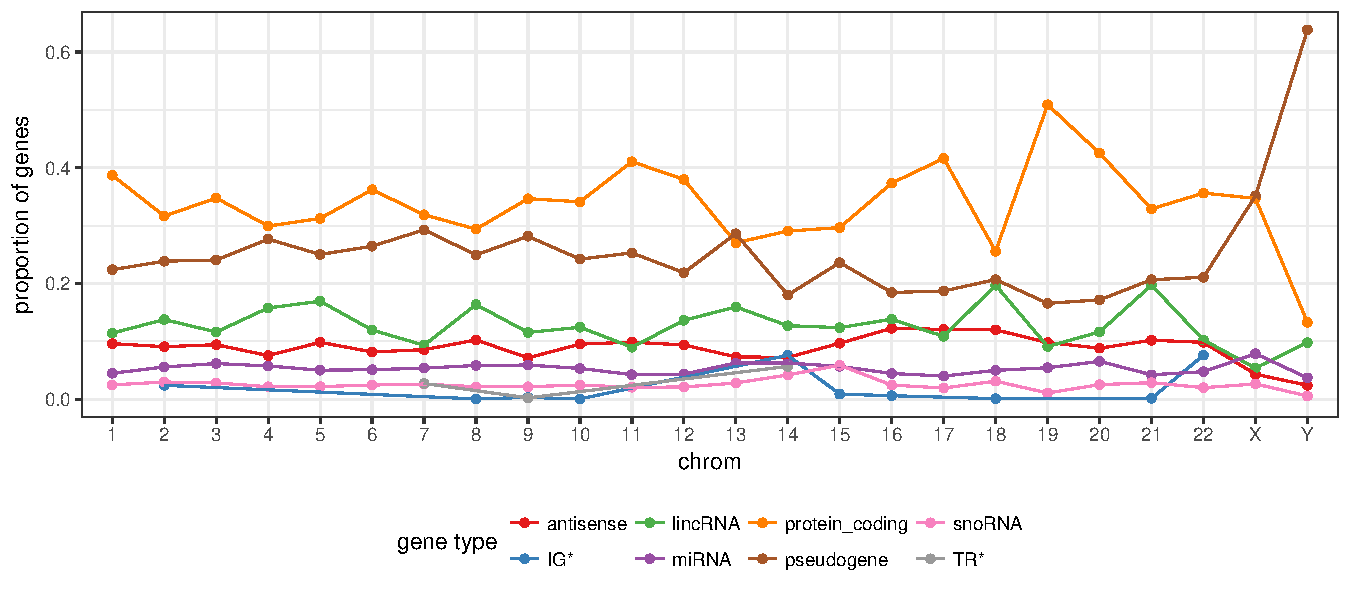
\includegraphics[height=.5\textheight]{../imgs/propGenesChr.pdf}

    {\it\scriptsize Tips: simplify (e.g. IG*/TR*) gene types and keep most common ones.}
  \end{enumerate}
\end{frame}

\begin{frame}[fragile]{Lunch Break}
  \begin{block}{Take-home messages}
    \begin{itemize}
    \item \verb!fread! instead of \verb!read.table!.
    \item \verb!lapply! instead of loops (also easy to parallelize).
    \item Functions instead of copy-pasting.
    \item \dfs and the Tidyverse for exploration and visualization.
    \end{itemize}
  \end{block}
  \begin{block}{More in appendix}
    \begin{itemize}
    \item Reading a file chunk by chunk.
    \item Working with file slices for BED/VCF/BAM files using indexing.
    \item Using computing clusters in R.
    \end{itemize}
  \end{block}
\end{frame}

%%%%%%%%%%%%
%%%%%%%%%%%%
%%%%%%%%%%%%
%%%%%%%%%%%%
%%%%%%%%%%%%
%%%%%%%%%%%%
%%%%%%%%%%%%
%%%%%%%%%%%%
%%%%%%%%%%%%
%%\section{Bioconductor}

\begin{frame}[fragile]{GenomicRanges package}
  Genomic regions can be represented by {\it GRanges} objects. Used in many packages/analysis.
  \begin{block}{}
  \begin{lstlisting}
library(GenomicRanges)

## Creating GRanges
gr = GRanges('chr1:103-404')
gr = GRanges('chr1', IRanges(103, 404))
gr = makeGRangesFromDataFrame(df, keep.extra.columns = TRUE)

## Changing the chromosome labels
seqlevels(genc) = gsub("chr","",seqlevels(genc))
## or
seqlevels(genc) = paste0("chr",seqlevels(genc))

## Other
width(gr)
promoters(gr)
resize(gr, width=width(gr)+1000, fix='center')
  \end{lstlisting}
  \end{block}
\end{frame}

\begin{frame}[fragile]{AnnotationHub}
  The \href{http://bioconductor.org/packages/release/bioc/html/AnnotationHub.html}{AnnotationHub} package allows you to access genomic files and anotations (e.g. UCSC files, Epigenome RoadMap, Encode).
  \bigskip
  
  \begin{itemize}
  \item \verb!query! function to search/list resources.
  \item Download by accessing the element.
  \item Eventually, \verb!import! to import BigWig files.
  \end{itemize}
  \begin{block}{}
  \begin{lstlisting}
library(AnnotationHub)
ah = AnnotationHub()
his.q = query(ah, c('Gm12878','H3K4me3','hg19'))
his.gr = his.q[[1]]

## If BigWig file, import only relevant region.
his.gr = import(his.q[[1]], which=reg.gr)
  \end{lstlisting}
  \end{block}  
\end{frame}

\begin{frame}[fragile]{Exercise}
  \begin{enumerate}
  \item Create a {\it GRanges} with the protein-coding genes in chr 1.
  \item Create a {\it GRanges} with the promoters protein-coding genes in chr 1. Promoter regions must be 1bp-long.
    \bigskip
  \item Find and download broad H3K4me3 peaks for Gm12878.
    \bigskip
  \item Find and download CpG islands for Hg19.
  \item Expand CpG islands by 10 Kbp using the \verb!resize! function.
    \bigskip
  \item Find and download Whole Genome Bisulfite Sequencing methylation data for Hg19.
  \item Retrieve methylation information around 1000 randomly selected CpG islands (from question 5).
  \end{enumerate}
\end{frame}

\begin{frame}[fragile]{Enrichment heatmaps}
  Bioconductor package \href{http://bioconductor.org/packages/release/bioc/vignettes/EnrichedHeatmap/inst/doc/EnrichedHeatmap.html}{EnrichedHeatmap} creates heatmap of overlaps between two {\it GRanges}. Typical example: Binding sites on known domains.

  \begin{exampleblock}{Example}
\begin{lstlisting}
mathm = normalizeToMatrix(H3K4me3, tss, value_column = "coverage", extend = 5000, mean_mode = "w0", w = 50)
EnrichedHeatmap(mathm, name = "H3K4me3")

mathm = normalizeToMatrix(meth, cgi, value_column = "meth", mean_mode = "absolute", extend = 5000, w = 50, background = NA)
EnrichedHeatmap(mathm)
\end{lstlisting}
  \end{exampleblock}  
  \begin{alertblock}{Exercise}
    \begin{enumerate}
    \item Heatmap of the histone mark around genes promoters in chr 1.
    \item Heatmap of the methylation level in and around the 1000 random CpG islands.
    \end{enumerate}
  \end{alertblock}
\end{frame}

\begin{frame}[fragile]{Overlaps between two {\it GRanges} sets}
  \begin{block}{Which function fit your exact need ?}
    \begin{description}
    \item[overlapsAny] Test overlaps of one \gr into second \gr.
      \medskip
    \item[countOverlaps] For each region in one \gr, count how many overlaps from another.
      \medskip
    \item[findOverlaps] Finds overlaps between two {\it GRanges} objects.
      \medskip
    \item[distanceToNearest] Computes the distance from each regions in a {\it GRanges} object to the nearest in another {\it GRanges} object.
      \medskip
    \item[subsetByOverlaps] Keep the regions from one \gr that overlaps another.
    \end{description}
  \end{block}
\end{frame}

\begin{frame}[fragile, shrink=10]{Overlaps between two {\it GRanges} sets}
  \begin{block}{{\sf findOverlaps} function}
    \begin{itemize}
    \item Two {\it GRanges} objects as input.
    \item Extra parameters available for specific overlaps.
    \item Returns the index of regions in object 1 and 2 that overlap.
    \item \verb!queryHits! and \verb!subjectHits! functions to retrieves those index.
    \end{itemize}
  \end{block}
  \begin{exampleblock}{Example}
\begin{lstlisting}
> ol12 = findOverlaps(gr1, gr2)
> ol12
Hits of length 3
queryLength: 6
subjectLength: 4
  queryHits subjectHits
   <integer>   <integer>
 1         1           1
 2         2           2
 3         5           3
> queryHits(ol12)
[1] 1 2 5
\end{lstlisting}
  \end{exampleblock}

\end{frame}

\begin{frame}[fragile]{Better one big overlap than many small ones}
  \begin{alertblock}{Exercise}
    For each gene type, how many genes overlap an H3K4me3 histone mark in Gm12878 ?
  \end{alertblock}

  \begin{block}{Hints}
    \verb!lapply!, \verb!tapply!, {\it dplyr}, GRanges$\leftrightarrow$\df
  \end{block}
\end{frame}

\begin{frame}[fragile]{{\it GenomicRanges} + {\it dplyr}}
  Convert the results of \verb!findOverlaps! to a \df and pipe it to {\it dplyr}.
  \bigskip
  
  \begin{block}{}
  \begin{lstlisting}
findOverlaps(gr1, gr2) %>% as.data.frame %>% 
    mutate(col1=gr1$col1[queryHits], ...subjectHits...) %>% 
       group_by(col1) %>% summarize(...)
  \end{lstlisting}
  \end{block}
  \begin{alertblock}{Exercise}
    \begin{enumerate}
    \item In one pipe/line: For each gene type, how many genes overlap an H3K4me3 histone mark in Gm12878 ?
    \end{enumerate}
  \end{alertblock}

\end{frame}


\begin{frame}[fragile]{Gene Ontology enrichment}
  The \href{http://bioconductor.org/packages/release/bioc/html/clusterProfiler.html}{clusterProfiler} package provides functions for Gene Ontology enrichment and Gene Set Enrichment Analysis.
  \bigskip
  
  \begin{block}{}
\begin{lstlisting}
library(clusterProfiler)
library(org.Hs.eg.db)

go.enr = enrichGO(gene=sig.entrez, 'org.Hs.eg.db', ont="BP", 
   universe=all.entrez, readable=TRUE)

go.enr.s = as.data.frame(go.enr)
head(go.enr.s[,c("Description","GeneRatio","qvalue")],20)

## With gene names (in theory)
go.enr = enrichGO(gene=sig.symbol, 'org.Hs.eg.db', ont="BP", 
   universe=all.symbol, readable=TRUE, keyType='SYMBOL')
\end{lstlisting}
  \end{block}
\end{frame}

\begin{frame}[fragile]{Convert gene names to Entrez IDs}
  Some functions work better with Entrez IDs.
  \bigskip
  
  \begin{block}{}
\begin{lstlisting}
library(clusterProfiler)
library(org.Hs.eg.db)

conv.df <- bitr(gene.symbols, fromType = "SYMBOL",
        toType = c("ENTREZID"),
        OrgDb = org.Hs.eg.db)

symbolToEntrez = conv.df$ENTREZID
names(symbolToEntrez) = conv.df$SYMBOL

sig.entrez = symbolToEntrez[sig.symbol]
\end{lstlisting}
  \end{block}
\end{frame}

\begin{frame}[fragile]{Exercise}
  \begin{enumerate}
  \item Find genes overlapping H3K4me3 marks with a score larger than 900.
  \item GO enrichment analysis on these genes.
    \bigskip
  \item If you get an error (or for ``fun''), try to convert the gene names to Entrez IDs.
  \end{enumerate}
\end{frame}

\begin{frame}[fragile]{{\it Gviz} for multi-track graphs}
  \begin{block}{}
  \begin{lstlisting}
library(Gviz)

region.gr = GRanges('chr3:110e6-116e6')
annot.reg.gr = subsetByOverlaps(annot.all.gr, region.gr)
data.reg.gr = subsetByOverlaps(data.all.gr, region.gr)

ga.t = GenomeAxisTrack()
annot.t = AnnotationTrack(annot.reg.gr, name = "Annot", feature=annot.reg.gr$color, group=annot.reg.gr$name)
data.t = DataTrack(data.reg.gr, data="score", type='h', name="Data")

plotTracks(list(ga.t, annot.t, data.t), showId=TRUE, my_feature_name='red')
  \end{lstlisting}

  \end{block}

  \begin{block}{More info}
    See slides/code/links from \href{https://github.com/jmonlong/MonBUG17_Gviz}{MonBUG Gviz demo}.
  \end{block}

  \begin{alertblock}{Exercise}
    Try to make a graph of the gene annotation and histone mark scores in chr3 between 110 Mbp and 116 Mbp.
  \end{alertblock}

\end{frame}

\end{frame}

\begin{frame}{Final recommendations}
  \begin{itemize}
  \item Use \textbf{names} that makes sense (to you and future you).
  \item \textbf{Nothing in the console}, everything in an organized script.
  \item The script should be \textbf{sequential and commented} when complex.
  \item Save the graphs \textbf{in the code}, not manually through RStudio.
  \item \textbf{Split} long scripts and \textbf{save} temporary files.
  \item \textbf{Overwriting} objects is fine if in the same paragraph.
  \item Use \textbf{functions/pipes} to avoid environment/code pollution.
  \item Use \textbf{R Markdown} to produce a readable report while keeping the code.
  \end{itemize}
\end{frame}


\section{Appendix}

\begin{frame}[fragile]{Chunk-by-chunk approach}
  \begin{block}{}
    When you can analyze the data in slices.
    \bigskip
    \begin{itemize}
    \item[+] Only a slice of the file in memory.
    \item[-] A bit painful/ugly.
    \end{itemize}
  \end{block}
\bigskip

\begin{block}{}
  \begin{lstlisting}
con = file(file.name)
while(length((chunk.df = read.table(con,nrows=1000)))>0){
... Instructions
}
close(con)
\end{lstlisting}
\end{block}
\end{frame}

\begin{frame}[fragile]{Bioconductor packages}
  \begin{block}{}
    \begin{itemize}
    \item GFF format with \verb!import! ({\it rtracklayer} package).
    \item VCF format with \verb!readVcf! ({\it VariantAnnotation} package).
    \end{itemize}
  \end{block}
  \begin{block}{}
    \begin{description}
    \item[+] Parse the format.
    \item[-] Sometimes parse too much $\rightarrow$ complicated object.
    \item[+] Read indexed files.
    \end{description}
  \end{block}

  \begin{alertblock}{Exercise}
    \begin{enumerate}
    \item Read \verb!gencode.gtf.gz! in another object using \verb!import!.
    \item Have a look at the data.
    \end{enumerate}
  \end{alertblock}
\end{frame}

\begin{frame}{Using file indexing}
  \begin{block}{Why indexing ?}
    To \textbf{quickly import a slice} of a file. In genomics, one region.
  \end{block}
  \bigskip
  \begin{block}{Indexing workflow}
    \begin{enumerate}
    \item Order file by position (chr + start).
    \item Compress with bgzip.
    \item Index.
    \end{enumerate}
  \end{block}
  \bigskip
  \begin{block}{How ?}
    With command lines or with R functions.
  \end{block}
\end{frame}

\begin{frame}[fragile]{Indexing files with R}
  \begin{block}{}
    {\it data.table} package is faster to order large files than conventional R.
  \end{block}
  \bigskip
  \begin{block}{}
  \begin{lstlisting}
library(data.table)
dt = fread("file.bed")
setkey(dt, chr, start)
write.table(dt, file="file-ordered.bed")

library(Rsamtools)
bgzip("file-ordered.bed")
indexTabix("file-ordered.bed.bgz")
  \end{lstlisting}
  \end{block}
\end{frame}

\begin{frame}[fragile]{Using indexed files}
  \begin{block}{}
  \begin{lstlisting}
reg = GRanges(...)

library(VariantAnnotation)
vcf <- readVcf("variants.vcf.gz", "hg19", reg)

library(rtracklayer)
gtf = import(TabixFile("annotation.gtf.bgz"), which=reg)
  \end{lstlisting}
  \end{block}
  \bigskip
  \begin{alertblock}{Exercise}
  \begin{enumerate}
  \item Read variants in VCF between coordinates 30 Mb and 31 Mb.
  \item Order, write, compress and index the gencode file.
  \item[$\divideontimes$] Tile the Mb in 10 bins. In each bin count the number of variants in the VCF.
  \end{enumerate}
  \end{alertblock}
\end{frame}

\begin{frame}{Using computing clusters directly with {\it BatchJobs}}
  \begin{block}{What you need}
    \begin{itemize}
    \item A function that can independently the code
      \begin{itemize}
      \item Load packages.
      \item Load necessary data.
      \item Run the code.
      \end{itemize}
    \item A parameter list (used to define the jobs).
    \item Some global objects (same for all jobs). Optional.
    \item Your favorite cluster configured (or your computer).
    \end{itemize}
  \end{block}
  \begin{block}{More info}
    Checkout \href{http://jmonlong.github.io/PopSV//2-ClusterManagement.md/}{PopSV documentation on BatchJobs}. To use Guillimin, Abacus, Briaree or Mammouth \href{mailto:jean.monlong@mail.mcgill.ca}{ask me} for the configuration files.
  \end{block}
\end{frame}

\begin{frame}[fragile]{BatchJobs example}

  \begin{lstlisting}
library(BatchJobs)

reg = makeRegistry("perm")

jobFun <- function(ii, necessaryData){
    library(...)
    ... Instructions using 'ii' and 'necessaryData'
    data.frame(perm=ii, ...)
}

batchMap(reg, jobFun, 1:10, more.args=list(necessaryData=myData))

submitJobs(reg))

showStatus(reg)

perm.l = reduceResultsList(reg)
  \end{lstlisting}

\end{frame}

\begin{frame}[fragile]{Heatmaps}
  \verb!heatmap! built-in function: heatmap, dendogram, one information annotation for the columns/rows.
  \bigskip

  \centering
  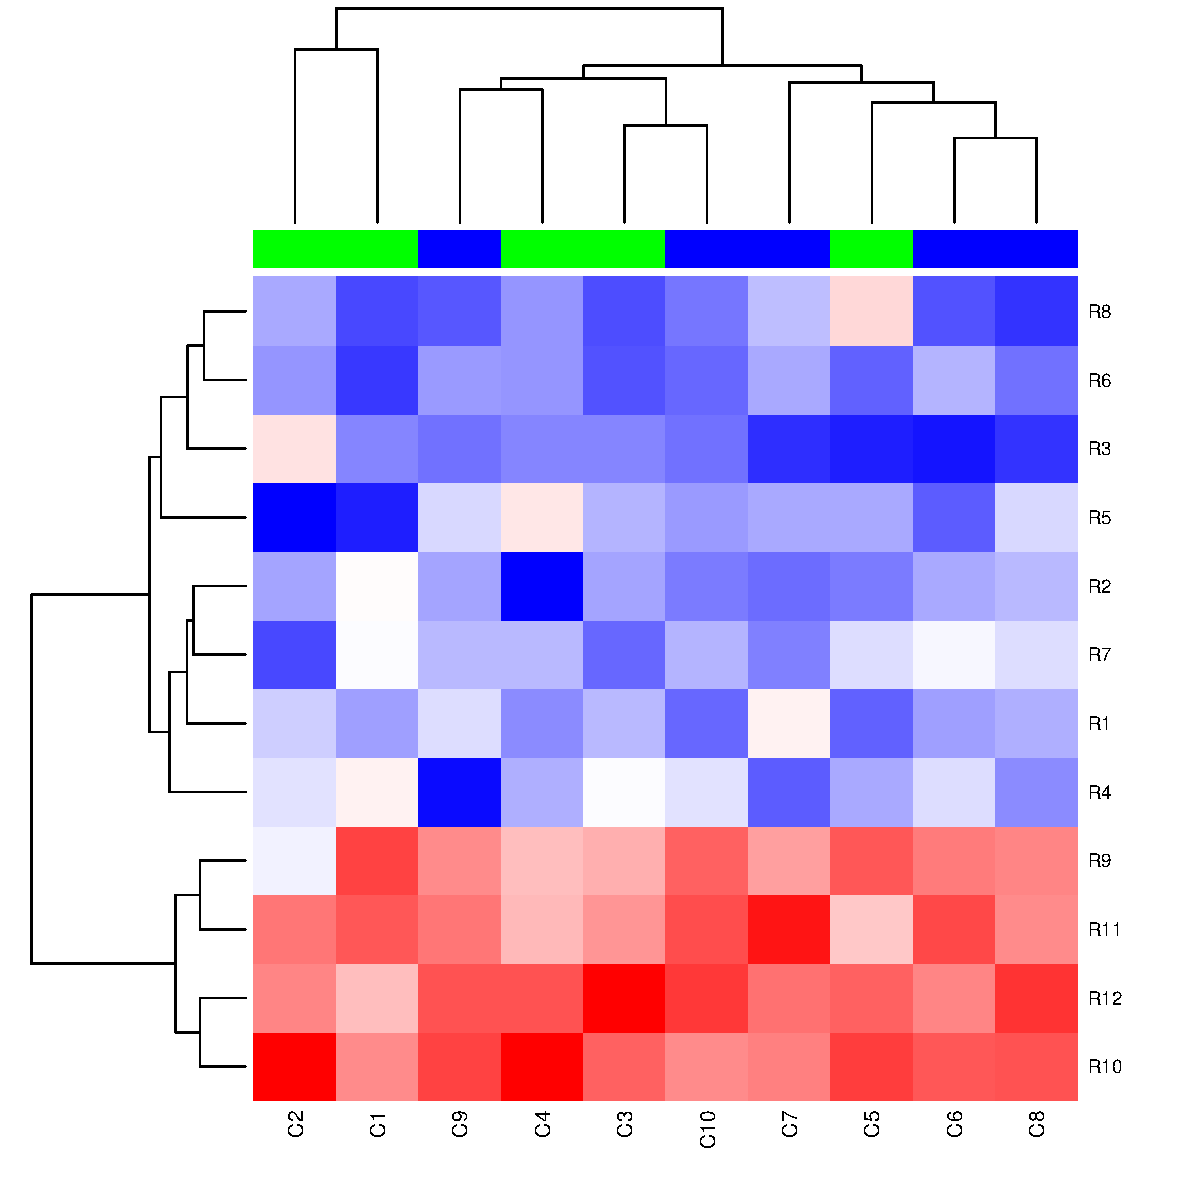
\includegraphics[height=.8\textheight, page=1]{../imgs/heatmaps.pdf}

\end{frame}

\begin{frame}[fragile]{Heatmaps}
  \verb!heatmap.2! function from {\it gplots} package: density distribution in legend and heatmap.
  \bigskip

  \centering
  \includegraphics[height=.8\textheight, page=2]{../imgs/heatmaps.pdf}

\end{frame}

\begin{frame}[fragile]{Heatmaps}
  \verb!Heatmap! function from {\it ComplexHeatmap} package: more columns/rows annotation with graphs and panels.
  \bigskip

  \centering
  \includegraphics[height=.8\textheight, page=3]{../imgs/heatmaps.pdf}

\end{frame}

\end{document}


%%% Local Variables:
%%% mode: latex
%%% TeX-master: t
%%% End:
